\documentclass{article}


\usepackage[utf8]{inputenc}
\usepackage{graphicx}
\usepackage{subcaption}
\usepackage[T1]{fontenc}
\usepackage{hyperref}
\usepackage{url}
\usepackage{booktabs}
\usepackage{amsfonts}
\usepackage{nicefrac}
\usepackage{microtype}
\usepackage{xcolor}
\usepackage{lipsum}
\usepackage{amsmath}
\usepackage{pdfpages}
\usepackage{float}

\newcommand{\note}[1]{\textcolor{blue}{{#1}}}
% Define a custom command for placeholders
\newcommand{\figureplaceholder}[2]{%
    \begin{figure}[H]
        \centering
        \fbox{\parbox{\dimexpr\linewidth-2\fboxsep-2\fboxrule\relax}{%
            \centering
            \textbf{Placeholder for Figure: #1}\\
            \emph{Description: #2}%
        }}
        \caption{#2}
        \label{fig:#1}
    \end{figure}
}
\title{
  Emotion Classification in Texts using Traditional Machine Learning and BERT \\
  \vspace{1em}
}

\author{
    Zhang Yibing 123090837\\
    School of Data Science \\
    Chinese University of Hong Kong, Shenzhen \\
  \texttt{yibingzhang@link.cuhk.edu.cn} \\
}

\begin{document}

\maketitle

\section{Introduction and Related Work}

Emotion recognition in text is a critical NLP task \cite{murthy2021}, classifying text into categories such as \textbf{joy, sadness, anger, fear, and neutral} \cite{acheampong2020}. This field has seen advancements from traditional machine learning methods to modern contextual models \cite{aman2007}. Analyzing the emotional cues implied in the text also greatly promotes the development of the language model \cite{alm2005}. This project compares two approaches using a \textbf{publicly available online corpus}: 1) Traditional Machine Learning (ML) with TF-IDF and classical classifiers (NB, LR, RF, SVM), and 2) a state-of-the-art Deep Learning approach using the \textbf{BERT} transformer model. This comparative study highlights the performance trade-offs between feature-engineered ML models and highly contextual, pre-trained transformers.

\section{Approach}
\subsection{Traditional Machine Learning Pipeline}
Text preprocessing used \texttt{spaCy} for cleaning, lemmatization, and stop word removal. Features were extracted using \texttt{TfidfVectorizer} with \textbf{Unigrams and Bigrams} ($\text{ngram\_range}=(1, 2)$). The vectorizer was fitted on the entire corpus (7,934 texts). Four classifiers \textbf{(Multinomial Naive Bayes (NB), Logistic Regression (LR), Random Forest (RF), and Linear Support Vector Classifier (SVC))} were trained and evaluated on the test set.

\subsection{Deep Learning Pipeline (BERT)}
The BERT model was initialized via the \texttt{ktrain} library. The input text was tokenized and formatted with a maximum length of 350. The model was fine-tuned using the \textbf{one-cycle learning rate schedule} for \textbf{3 epochs} with a max learning rate of $2e-5$. This approach leverages BERT's contextual embeddings, eliminating manual feature engineering.

\section{Experiments}
\subsection{Data and Evaluation Method}
The dataset was sourced from a publicly available corpus, split into a Training Set (7,934 texts) and a Test Set (3,393 texts). The five emotion classes are primarily balanced (e.g., 'joy' is $\approx 2,326$, 'fear' is $\approx 2,171$). Performance was primarily measured using the \textbf{micro-averaged F1 Score} and \textbf{Accuracy} on the test set.

\subsection{Experiment Results and Analysis}

\subsubsection{Performance Comparison}
The performance metrics for both traditional ML and BERT are summarized in Table \ref{tab:results_summary}.


The \textbf{Logistic Regression} achieved the highest score among traditional models, demonstrating robustness in the high-dimensional TF-IDF space. However, the \textbf{BERT} model significantly outperformed all traditional methods, achieving a $82.42\%$ F1-Score. This \textbf{$14.01\%$ point gain} confirms the superior ability of transformer models to capture complex emotional context over simple bag-of-words (TF-IDF) representations.

\subsubsection{Confusion Matrix Analysis}
The normalized confusion matrices (Figure \ref{fig:confusion_matrices}) illustrate class-specific performance. All traditional models consistently showed difficulty in distinguishing between \textbf{sadness} and \textbf{neutral}, and between \textbf{joy} and \textbf{neutral}.


\section{Conclusion}

This comparative study demonstrated that while the \textbf{Logistic Regression} achieved a strong baseline (F1: $68.41\%$) on the emotion classification task using TF-IDF features, the \textbf{BERT} transformer model achieved state-of-the-art performance (F1: $82.42\%$). The substantial performance gap validates the shift towards pre-trained contextual models in modern NLP for tasks requiring nuanced semantic understanding. Both the optimal traditional pipeline (TF-IDF + SVM) and the fine-tuned BERT model were successfully saved for deployment.



\bibliographystyle{unsrt}
\bibliography{references}

\appendix

\section{Appendix}

\begin{table}[H]
    \centering
    \caption{Summary of Classification Results}
    \label{tab:results_summary}
    \small % Use small font for table content
    \begin{tabular}{lcc}
        \toprule
        Approach & Accuracy ($\%$) & F1-Score ($\%$) \\
        \midrule
        Naive Bayes & 62.81 & 62.81 \\
        Random Forest & 65.69 & 65.69 \\
        \textbf{Logistic Regression} & \textbf{68.41} & \textbf{68.41} \\
        SVM (Linear) &  67.40 & 67.40 \\
        \midrule
        \textbf{BERT} & \textbf{82.42} & \textbf{82.42} \\
        \bottomrule
    \end{tabular}
\end{table}

\begin{figure}[H]
    \centering
    
    \begin{subfigure}[b]{0.49\textwidth} 
        \centering
        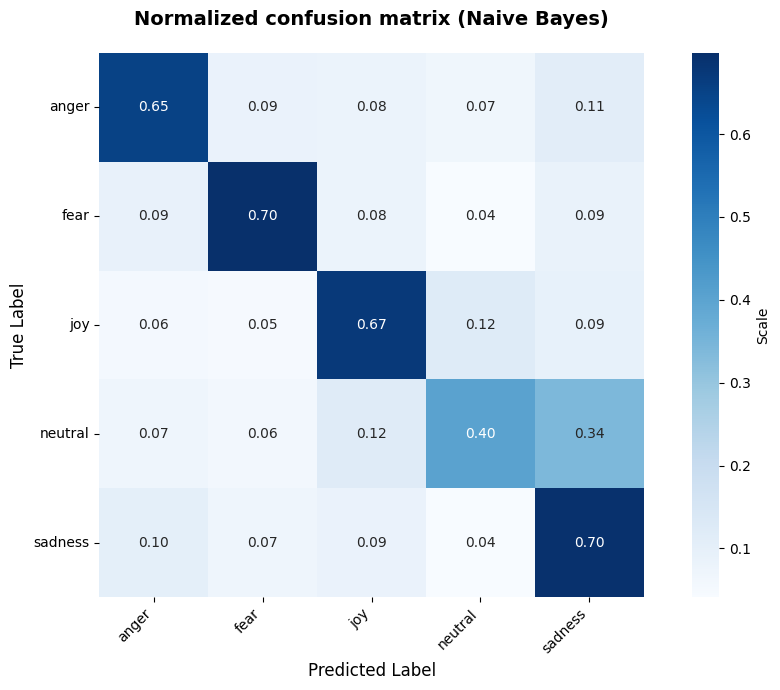
\includegraphics[width=0.94\textwidth]{nb_confusion_matrix.png} 
        \caption{Normalized CM (Naive Bayes)}
        \label{fig:nb_cm}
    \end{subfigure}
    \hfill 
    \begin{subfigure}[b]{0.49\textwidth}
        \centering
        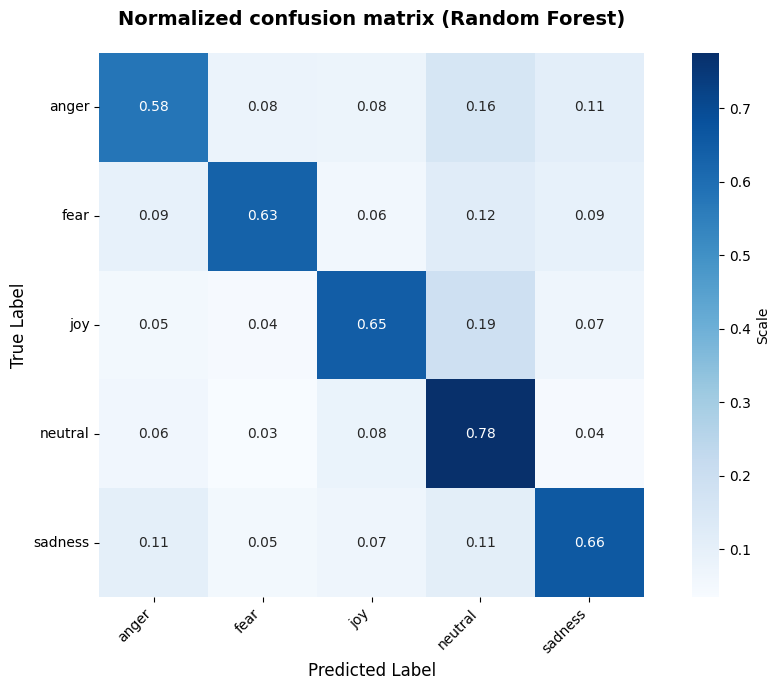
\includegraphics[width=0.94\textwidth]{rf_confusion_matrix.png} 
        \caption{Normalized CM (Random Forest)}
        \label{fig:rf_cm}
    \end{subfigure}
    
    \vspace{0.3cm} 
    
    \begin{subfigure}[b]{0.49\textwidth}
        \centering
        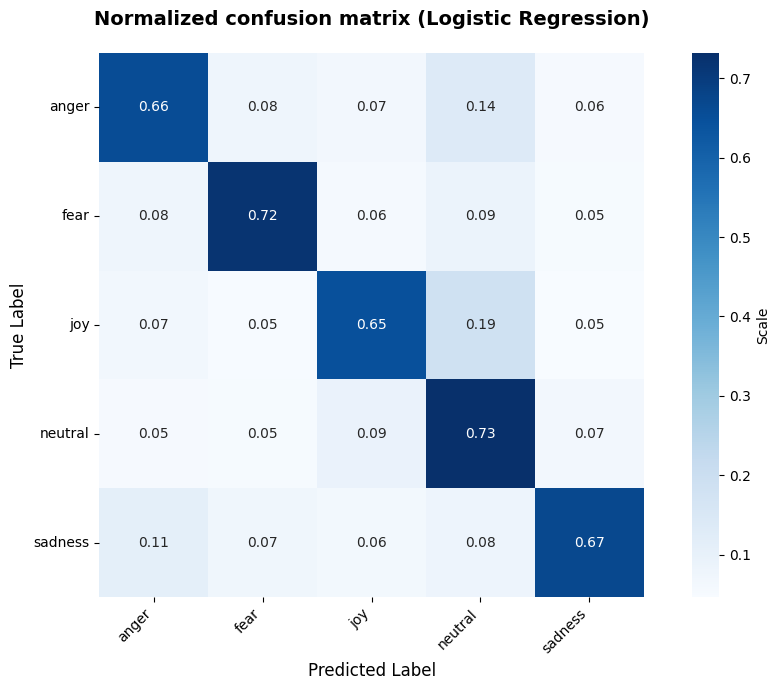
\includegraphics[width=0.94\textwidth]{lr_confusion_matrix.png} 
        \caption{Normalized CM (Logistic Regression)}
        \label{fig:log_cm}
    \end{subfigure}
    \hfill 
    \begin{subfigure}[b]{0.49\textwidth}
        \centering
        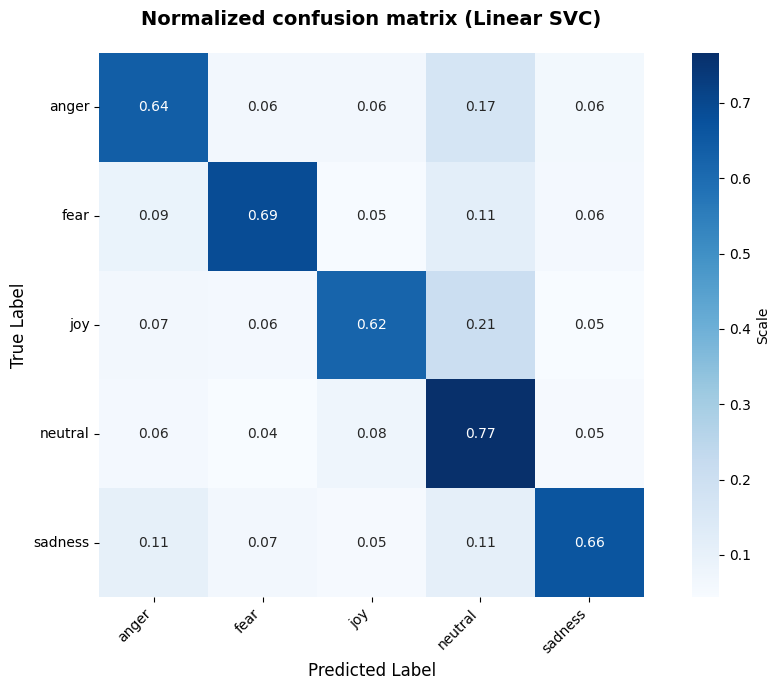
\includegraphics[width=0.94\textwidth]{svc_confusion_matrix.png} 
        \caption{Normalized CM (Linear SVC)}
        \label{fig:svc_cm}
    \end{subfigure}
    
    \caption{Normalized Confusion Matrices for Traditional Models.}
    \label{fig:confusion_matrices}
\end{figure}

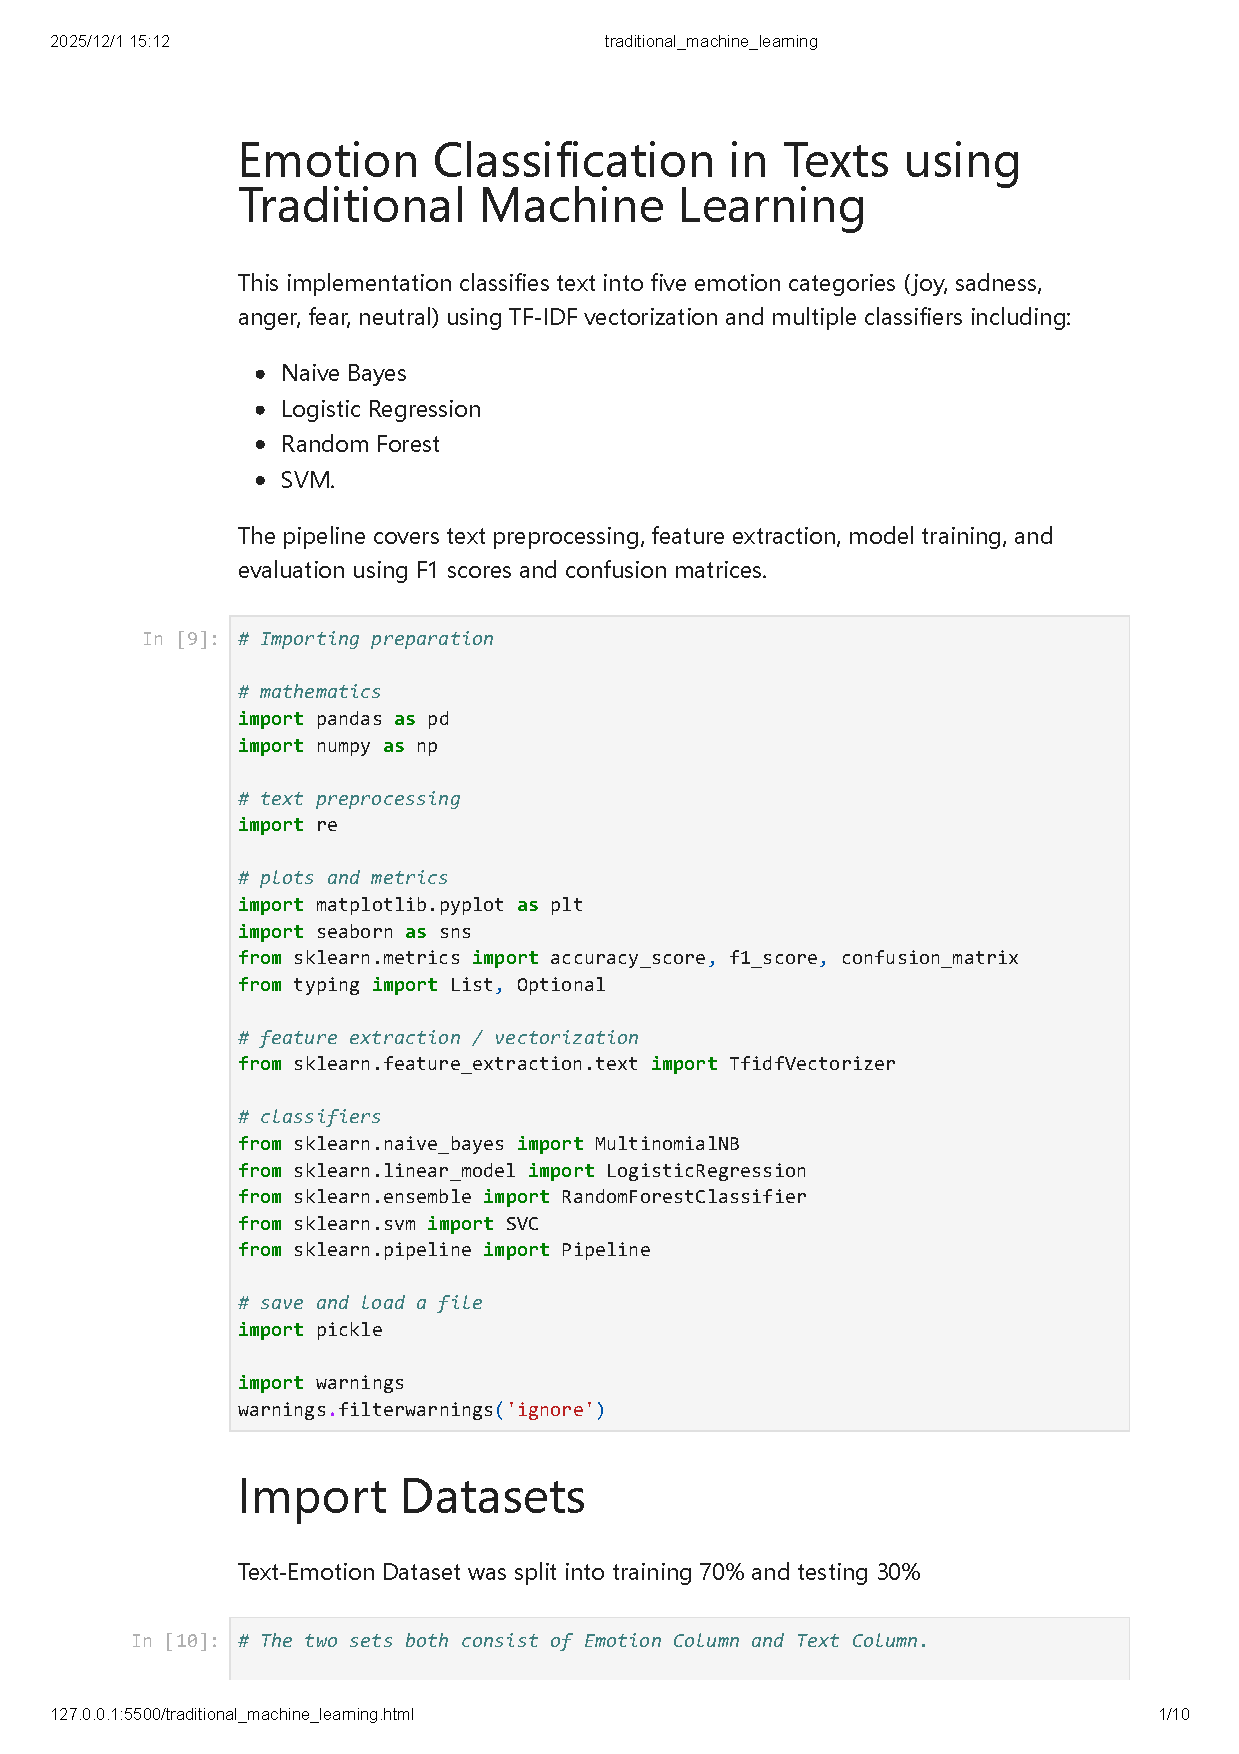
\includepdf[pages=-]{traditional_machine_learning.pdf}
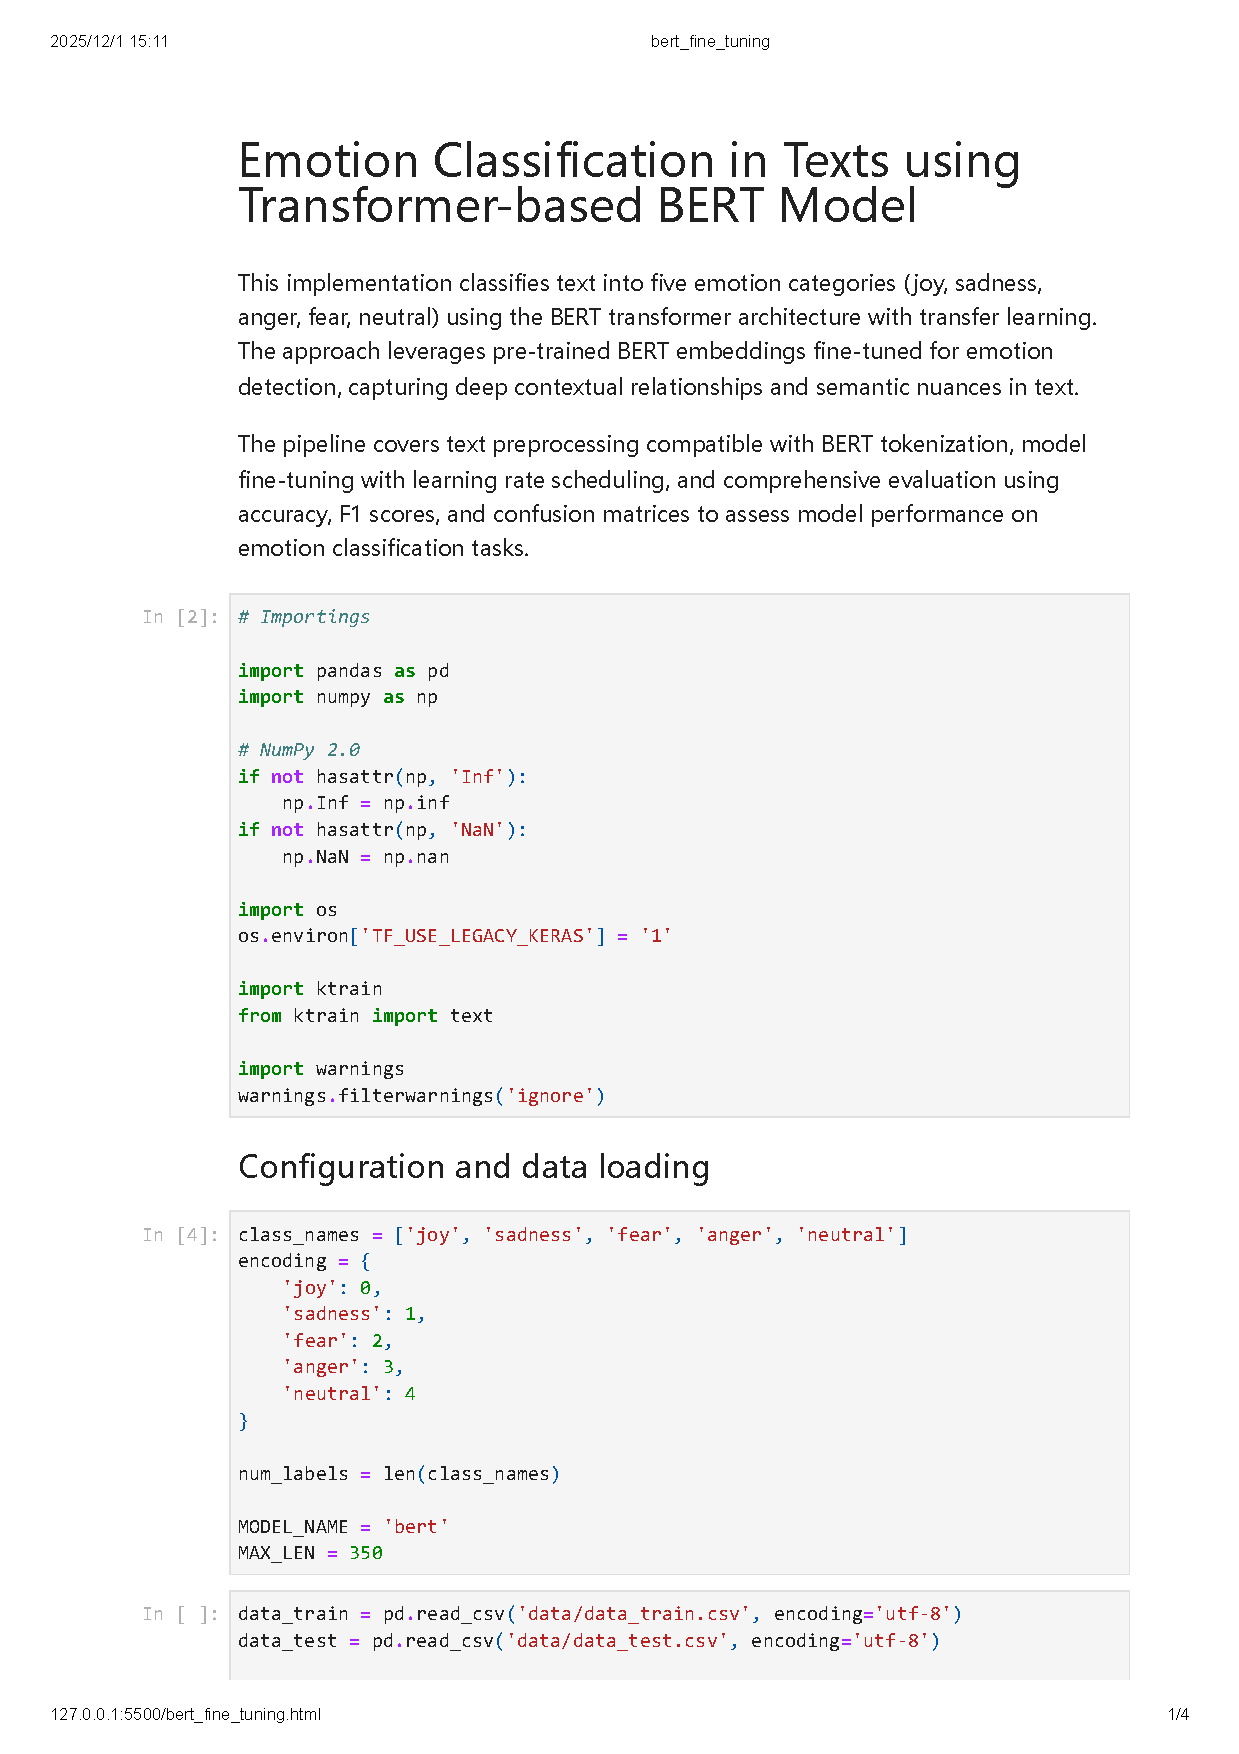
\includepdf[pages=-]{bert_fine_tuning.pdf}
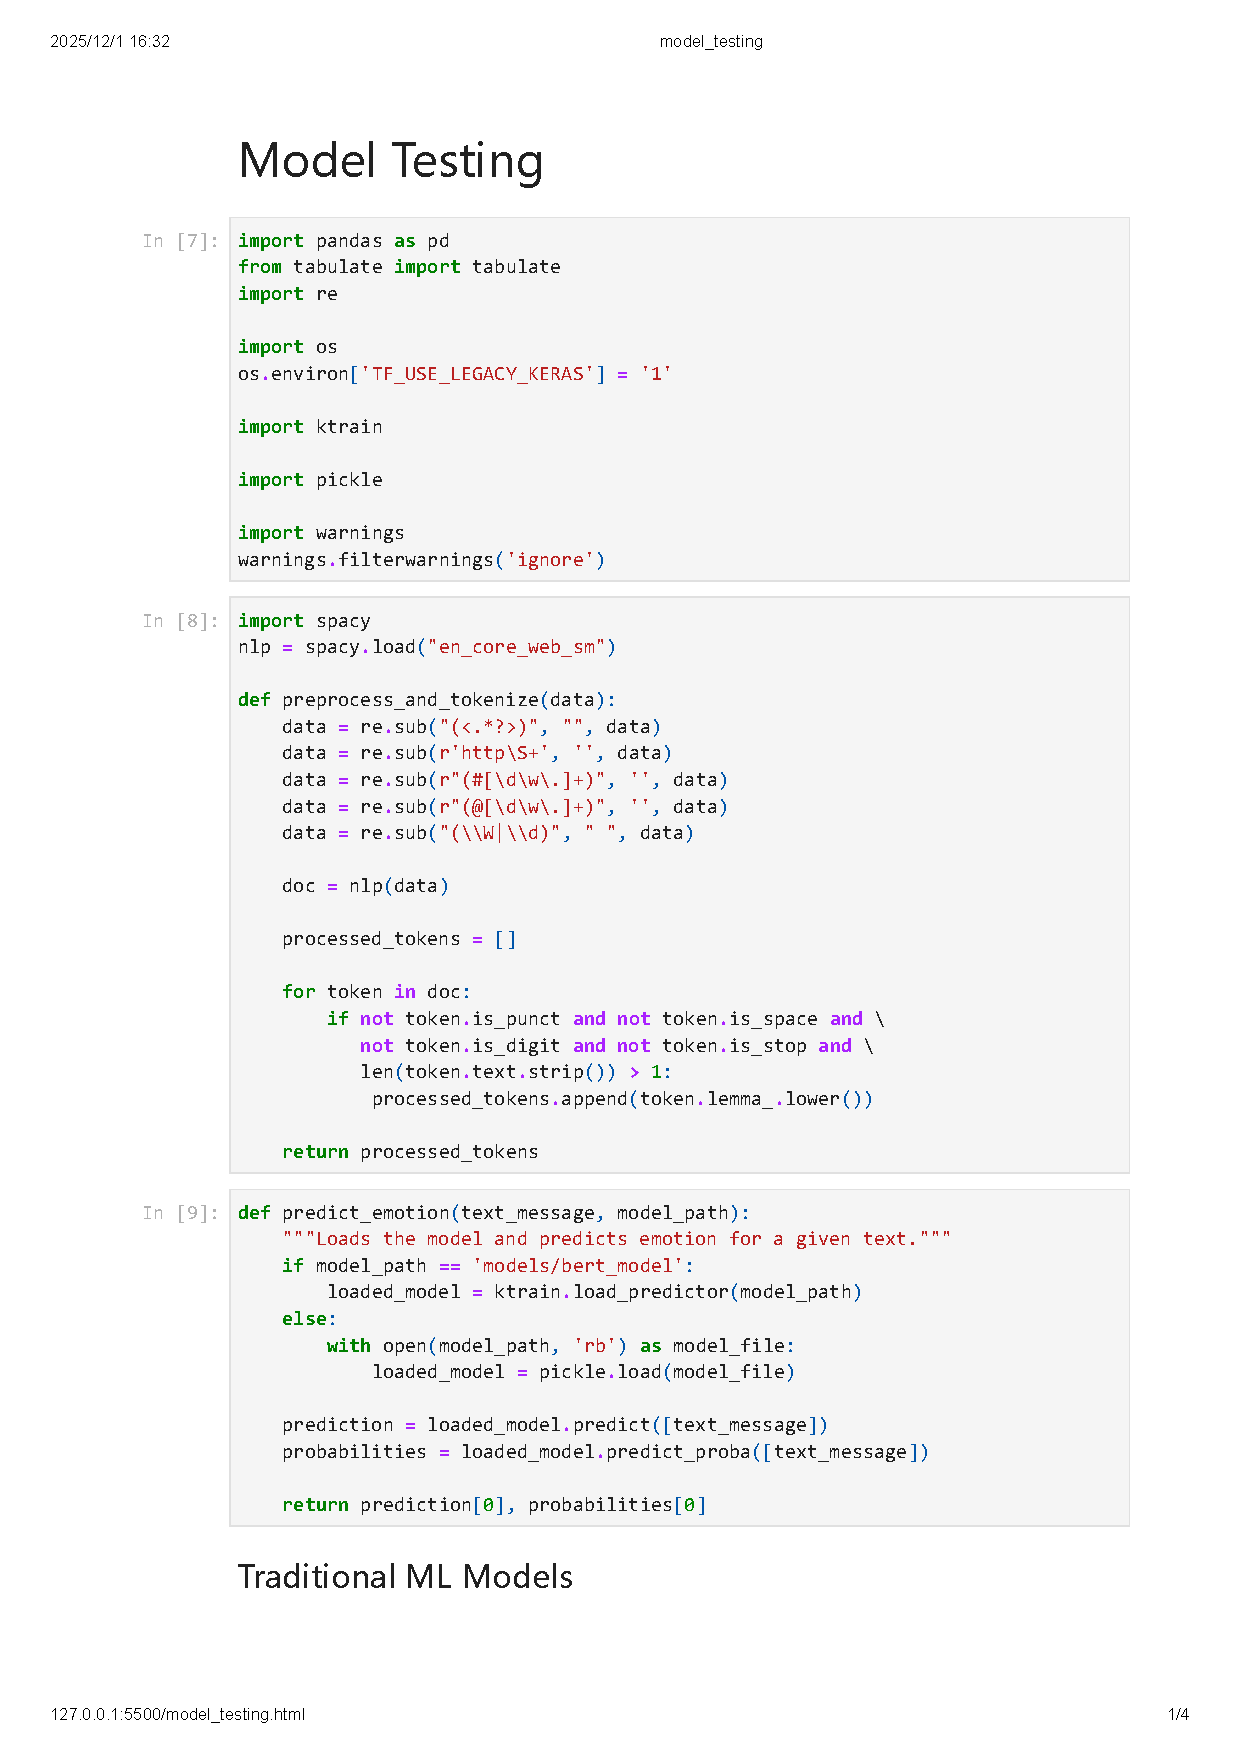
\includepdf[pages=-]{model_testing.pdf}

\section{References}
\begin{thebibliography}{99} % {99} 表示最大的引用编号是两位数

% [Murthy & Kumar 2021]
\bibitem{murthy2021}
Murthy, A. R., \& Kumar, K. A. (2021, March). A review of different approaches for detecting emotion from text. In \textit{IOP Conference Series: Materials Science and Engineering} (Vol. 1110, No. 1, p. 012009). IOP Publishing.

% [Acheampong et al. 2020]
\bibitem{acheampong2020}
Acheampong, F. A., Wenyu, C., \& Nunoo‐Mensah, H. (2020). Text‐based emotion detection: Advances, challenges, and opportunities. \textit{Engineering Reports}, 2(7), e12189.

% [Aman & Szpakowicz 2007]
\bibitem{aman2007}
Aman, S., \& Szpakowicz, S. (2007, September). Identifying expressions of emotion in text. In \textit{International conference on text, speech and dialogue} (pp. 196-205). Berlin, Heidelberg: Springer Berlin Heidelberg.

% [Alm et al. 2005]
\bibitem{alm2005}
Alm, C. O., Roth, D., \& Sproat, R. (2005, October). Emotions from text: machine learning for text-based emotion prediction. In \textit{Proceedings of human language technology conference and conference on empirical methods in natural language processing} (pp. 579-586).

\end{thebibliography}


\end{document}

